\chapter{Data modelling in the VO} % (fold)
\label{cha:data_modelling_in_the_vo}

% - VO seeks common services and data interoperability
% 
% - Common services must satisfy typical astronomy tasks, plus new data
%   mining needs
% 
% - Common services, as shown before
%   - Images
%   - Spectra
%   - Multi-dimensional datasets (to be defined, extending one or other
%     previous services)
% 
% - Data interoperability, needs a MODEL of astronomical data and
%   operations, so that data and applications can adhere to it.
	
	\invisiblenote{
		mod•el |ˈmädl| 
		noun 
		• (in sculpture) a figure or object made in clay or wax, to be reproduced in 
		another more durable material. 
		2 a system or thing used as an example to follow or imitate : the law became a model for 
		dozens of laws banning non-degradable plastic products | [as adjective ] a model farm. 
		• a simplified description, especially a mathematical one, of a system or process, to 
		assist calculations and predictions : a statistical model used for predicting the survival rates 
		of endangered species. 
		4 a particular design or version of a product : trading your car in for a newer model.
	}
	
	The interoperability of tools and archives in the VO is only
	achievable by standardising the way datasets are accessed, and
	how the scientific data they contain is described. The first
	part is solved by means of standard access protocols, while the
	latter needs the development of suitable data models.
	
	 A data model can be defined as a complete description of the
	set of entities needed for information storage in a particular
	field, which specifies both the data being stored, and the
	relationships between them.
	
	 In this way, it can also be seen as the framework in which
	questions about the data (and metadata) ca be posed: only
	questions which can be answered regarding the information AND
	relationships encoded in the data model can be answered within
	the VO framework. And considered this way, a uniform,
	interoperable observation data model can be mapped into
	a uniform set of questions which can be answered within the VO.
	
	 Two main classes of data models are typically considered:
	
	\begin{description}
		\item[Domain data models] These are high-level descriptions
		of the entities to be taken into account in order to fully
		implement a data model. Particular attributes of the data
		entities involved are not set, except for those needed for
		establishing the relationship between entities.
		
		\item[Implementation model] Implementation-dependent
		description of the particular entities and attributes to be
		actually stored.
	\end{description}
	
	 VO data models need to be a mixture of the model types above:
	for the data models to be used across observations with
	different instruments, and with different scientific objectives
	in mind, a high-level description is needed. In addition, VO
	data models affect how data from observatories' archives are
	exposed through VO services, as the way such
	data are stored by the archive might differ from the IVOA
	standards. 
	However, there are
	particular attributes that need a precise description in order
	for the model to be useful, and to be able to implement it,
	so VO data models need to fix the kind of metadata they
	support.
	
	 Within the VO, data models apply not only directly to the
	scientific data, but to the metadata describing them. As the
	way to structure information depends on the application domain,
	VO data models describe astronomical datasets in a way that is
	as instrument independent as possible, to ensure that the same
	description can be used for data with different origins.
	Users must also be able to query those data models to be able
	to find datasets which comply with certain properties.
	
	\section{Elements of a data model} % (fold)
	\label{sec:data_model_elements}
	
		When defining a VO data model, we have to specify:
	
		\begin{description}
			\item[Entities] Being the data model building blocks,
			they group related attributes within a data model. They
			can be mapped to Classes in Object-Oriented Programming
			(OOP), or Elements in XML.
			
			 \item[Fields] They are the actual data elements of the
			model. They map to Attributes in OOP, and they can be
			mapped to Attributes or to Elements without children in
			XML.
			
			 \item[Relationships] The different entities and fields
			have hierarchical or relational relationships: an
			observation project has projected observations, and
			all entities which share a common project ID are
			related, for instance. For the data model to be
			uniquely defined those relationships must be made
			explicit.
			
			 \item[Cardinalities] The number of object instances
			allowed as part of a relationship. It is specified as
			a range of valid number of entities.
			For instance, an
			observation can be related to any number of data files,
			but it needs to be related at least with one, meaning
			that the cardinality of the Observation to Data files
			relationship would be specified as 1..*. For objects
			which can appear any number of times, including none,
			the cardinality is expressed as 0..*. Objects which are
			optional, but if present can appear just once have their 
			cardinality expressed as 0..1, and so on.
			
			 \item[Data types] For computers to be able to
			correctly interpret a data stream a Data type needs to
			be specified. For instance, object IDs could be
			Integers, but they are normally textual, so String data
			must be used. We could consider the restrictions which
			can be defined for complex data types in XML as part of
			the data typing.
			
			 \item[Units] No physical quantity can be specified
			without providing its units. Physical-data related
			Fields need Units to be specified, or Units have to be
			a fixed property of certain Fields, but they either
			need to exist as an implicit attribute of a particular
			field, or to have their own dedicated Field.
			
			 \item[Semantics] As observation metadata are related
			to real-world elements and quantities, VO data models
			also imply data semantics ---i.e., what is exactly meant
			in the real world by a particular field--- to avoid
			ambiguities. Most of VO semantics are provided via
			Unified Content Descriptors (UCDs) and UTypes.
		\end{description}

	% section data_model_elements (end)
	
	\section{Semantics, UCDs, UTypes and IVOA vocabularies} % (fold)
	\label{sub:ucds_and_utypes}
		\newcommand{\ucdurl}[0]
		{http://www.ivoa.net/Documents/latest/ UCDlist.html}
		UCDs are a controlled vocabulary\urlnote{\ucdurl}, under
		the supervision of the IVOA Semantics WG, which provides a
		list of \emph{atoms} which can be used to identify fields
		as corresponding to specific astronomical quantities. For
		instance, a field containing the Right Ascension can be
		identified by the UCD atom \texttt{pos.eq.ra}, while a
		photometric flux\footnote{Photometric flux is the
		integrated flux received within a particular band; in
		practice, it is the integral of the emitted flux weighed by
		the corresponding filter response.} in the \emph{V}
		band\footnote{The \emph{V} band is defined by a filter with
		central wavelength around 540 to 550~nm, and with Full
		Width Half-Maximum of 80 to 90~nm.} can be identified by
		juxtaposing
		the two UCD atoms \texttt{phot.flux; em.opt.V}. This
		provides both a unified vocabulary to identify any
		astrophysical quantity, and an automatic knowledge
		discovery tool for fields with arbitrary relationships. In
		fact, UCDs were born out of a joint CDS/ESO data mining
		effort~\cite{1999ASPC..172..379O}.
		
		 However, UCDs can only provide \emph{data kind}
		information, but not relationship information. In a sense,
		they are a kind of specialised \emph{unit}, complementary
		---orthogonal--- to physical units: in the same way that
		quantities with the same physical units can be very
		different in nature (i.e., both the decay time for an
		isotope and the oscillation period for a pendulum are both
		measured in seconds, but do not have any other physical
		connection), fields with identical UCDs can also be related
		to different real-word phenomena. In order to allow such
		deeper relationships to be expressed, and disambiguate
		metadata fields UTypes were born.
		
		 UTypes are created from a hierarchical data model by
		enumerating the different parents a particular field has in
		that hierarchy. For instance, a field containing the Right
		Ascension in equatorial coordinates for where an instrument
		was pointed to corresponds to the spatial coverage
		characterisation, in particular to the Location property,
		and thus it would sport a UType of
		\texttt{characterisation.coverage.spa\-tial.lo\-ca\-tion},
		the UCD would be \texttt{pos.eq.ra}, and its units could be
		any angular unit.
		
		\newcommand{\ivoasemanticswgurl}[0]
	{http://www.ivoa.net/cgi-bin/twiki/bin/view/ IVOA/IvoaSemantics}
		 But even with the help of units, UCDs and UTypes,
		sometimes it can be difficult to tag a particular piece of
		data with meaningful semantics, specially for data which
		does not have a direct place in a VO data model. For that
		we can borrow techniques from the Semantic Web (an effort
		for providing web documents with semantics, so that, for
		instance, a table of camera prices can be tagged so that
		software tools can identify in it prices, if possible
		belonging to digital cameras, even to particular brands),
		and provide one or more standardised astronomical
		vocabularies. The IVOA Semantics
		WG\urlnote{\ivoasemanticswgurl} has started recreating
		controlled vocabularies such as UCDs in Semantic Web form,
		and even the IAU thesaurus has been recreated in that
		way~\cite{Derriere:2008jo}. We will show how we are using
		them in the IRAM~30m archive in order to provide semantics
		to data related to antenna engineering terms.

	% section ucds_and_utypes (end)

	\section{Role of data models in the VO} % (fold)
	\label{sec:role_of_data_models_in_the_vo}
	
		We can identify in the VO four different phases, and we can
		see that in all of them data models play a central role:
	
		\begin{description}
			\item[Discovery] Datasets available in the VO have to
			be discoverable for them to appear automatically in VO
			tools. The VO Registry holds information regarding
			existing datasets so that they can be easily
			discovered. For this phase to be standardised, we need:
			data models for Resource metadata (ResDM), were a
			Resource is either a data provider, an authority, or a
			data service; a data model for Space-Time Coordinates
			(STC), so that coordinate-based, region-based or
			time-based searches can be performed; and a data model
			for dataset Characterisation (CharDM), so that searches
			on physical or instrumental properties are possible. In
			addition, the UCD and IVOA thesaurus (IVOAT) are
			relevant in this phase.
			
			\item[Evaluation] Datasets have to be evaluated in
			order to assess their applicability to the kind of
			analysis we might wish to perform; for instance, in
			order to do image mosaicing we need a certain
			coordinate overlap, and in order to do image stacking
			we need an almost complete overlap, and comparable
			resolutions. The main data model involved in this phase
			is the CharDM.
			
			\item[Data Access] There is an implicit data model in
			the IVOA data access protocols, the Data Access Layer
			(DAL), which is centred on targets (coordinates with
			tolerances/search radii), and uses several properties
			from the CharDM, such as the Coverage in several axes,
			and a streamlined form of the STC.
			
			\item[Transformation] When creating a new dataset, or
			transforming an existing one, a new CharDM instance
			needs to be created, one that characterises the
			union of the participating datasets. If the
			transformed data set is a spectrum, the Spectral data
			model (SpecDM) is needed both for obtaining the
			complete description of the original data and
			describing the transformed product. There is no
			existing data model yet for images or for more complex
			data within the VO. In addition, in order to trace the
			origin of the transformed image we would need to use a
			Provenance data model, that apart from being an
			integral part of the Observation data model (ObsDM), it
			should be built in a stand-alone form so that it can be
			applied to newly generated, non-observational data.
		\end{description}
	
	% section role_of_data_models_in_the_vo (end)
	
	\section{Data modelling diagrams} % (fold)
	\label{sec:data_modelling_diagrams}
	
		For specifying the aforementioned elements several
		notations exist, being the Unified Modelling
		Language\urlnote{http://www.uml.org/} (UML) by Rumbaugh,
		Jacobson, and Booch~\cite{Rumbaugh:1998:UMLRG} one of
		the most widely used. Some of the IVOA data models have
		been specified in terms of UML diagrams, and will be used
		when available.
		
		However, UML tools tend to be too onerous for data
		modelling when the data model is not going to be used to
		generate code for implementing that data model in memory,
		and we have resorted to simplified entity-relationship
		diagrams~\cite{1976atds....1....9C}, with specification of
		the cardinalities when they are not made explicit in the
		text, and relational attributes included in the diagrams.
	
	% section data_modelling_diagrams (end)
	
	\section{Existing IVOA data models} % (fold)
	\label{sec:existing_ivoa_data_models}
	
		We have talked about different data models in use within
		the VO. In this section we will review the data models most
		relevant to the development of observation related archive
		data models, and see what their implementation level is.
	
		\subsection{Observation} % (fold)
		\label{sec:the_ivoa_observation_model}
	
			The Observation Data Model 
			(ObsDM)~\cite{2005dmo..rept.....M}
			was started as an
			effort to create a common framework in which all kinds
			of astronomical observations could be described. In
			that regard, it can be thought of as a Domain model,
			but with a strong focus on the ability to perform
			queries on the stored observation metadata.
			
			 In words of its authors, each ObsDM instance
			\emph{describes a single dataset which may be [either]
			a dataset corresponding to an observation of the sky,
			[or] a dataset derived from many observations, [but]
			with the stipulation that the dataset is intended to
			be analysed independently of other datasets, and contains
			all the primary data needed for such analysis.}
			
			 The ObsDM tries to provide, in a first approximation,
			all metadata needed for data selection and retrieval,
			while being extensible to the more specific case of all
			the metadata needed by data analysis applications.
			
			 Figure~\ref{fig:fig_ObservationDM} shows the general
			model for observation as contained in the first draft
			of the ObsDM working draft.
			
			\begin{figure}[tbp]
				\centering
					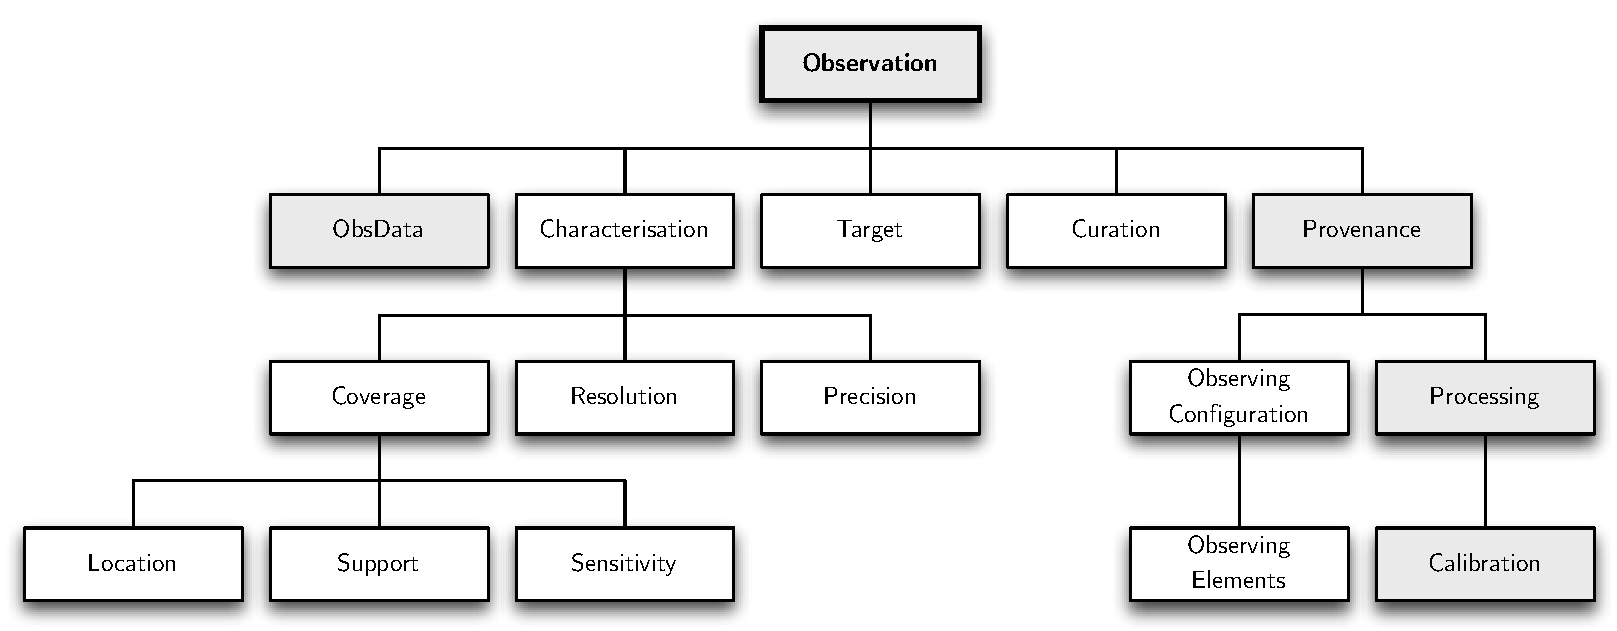
\includegraphics[width=\columnwidth]
					{fig/ObservationDM.pdf}
				\caption[The Observation Data Model]
				{
					 The Observation Data Model. Diagram recreated
					from the \emph{General Model for Observation}
					figure in the Data Model for Observation
					working draft~\cite{2005dmo..rept.....M} from
					2005. The shadowed rectangles show data and
					metadata items which can change in case of a
					reanalysis of the observational data,
					highlighting the essential difference between
					Provenance due to observing configuration setup
					and data processing. The hierarchical
					association does not show object
					cardinality, i.e., the number of times instances
					of an object can be related to its father
					object.
				}
				\label{fig:fig_ObservationDM}
			\end{figure}
			
			First, that figure shows that the main constituents
			of the ObsDM are the dataset Characterisation (where
			in parameter space can the observation be found),
			Target (what is known about the
			target of our observation), Curation (who is reponsible
			for getting this observation into the archive, or
			publishing it into the VO), and Provenance (what has
			been done to the set of photons which correspond to this
			observation).
			
			 The figure also illustrates the main difference between
			two different classes of Provenance: the metadata and
			data that would change in case of a reprocessing of 
			observed data are shadowed in grey. Neither the raw data
			themselves nor their characterisation would change,
			while the data provenance not having to do with the
			observational setup would have to reflect those changes.
			
			Another issue that can be derived from that figure is
			that the Characterisation is one of the most observation
			technique independent sub-data models of the
			Observation, and as such the work on the Observation
			data model was delayed until the Characterisation data
			model was finished.
			
			 We must note that even when the
			STC~\cite{2007stc..ivoa.....R}, and
			CharDM~\cite{2008dmadcrept.....L}, have reached the
			status of Recommendation, the
			ObsDM~\cite{2005dmo..rept.....M} is still an early
			working draft whose main role has been providing
			momentum to the STC and Characterisation efforts.
			\suppress[Enrique]{Once
			the CharDM reaches Recommendation status, the next
			efforts in order to complete the ObsDM are the
			Photometric data model (complementary to spectra), the
			Image data model, and the Provenance data model.}
		
		% subsection the_ivoa_observation_model (end)

		\subsection{Characterisation} % (fold)
		\label{sec:the_ivoa_characterisation_data_model}
			
			\begin{figure}[tbp]
				\centering
					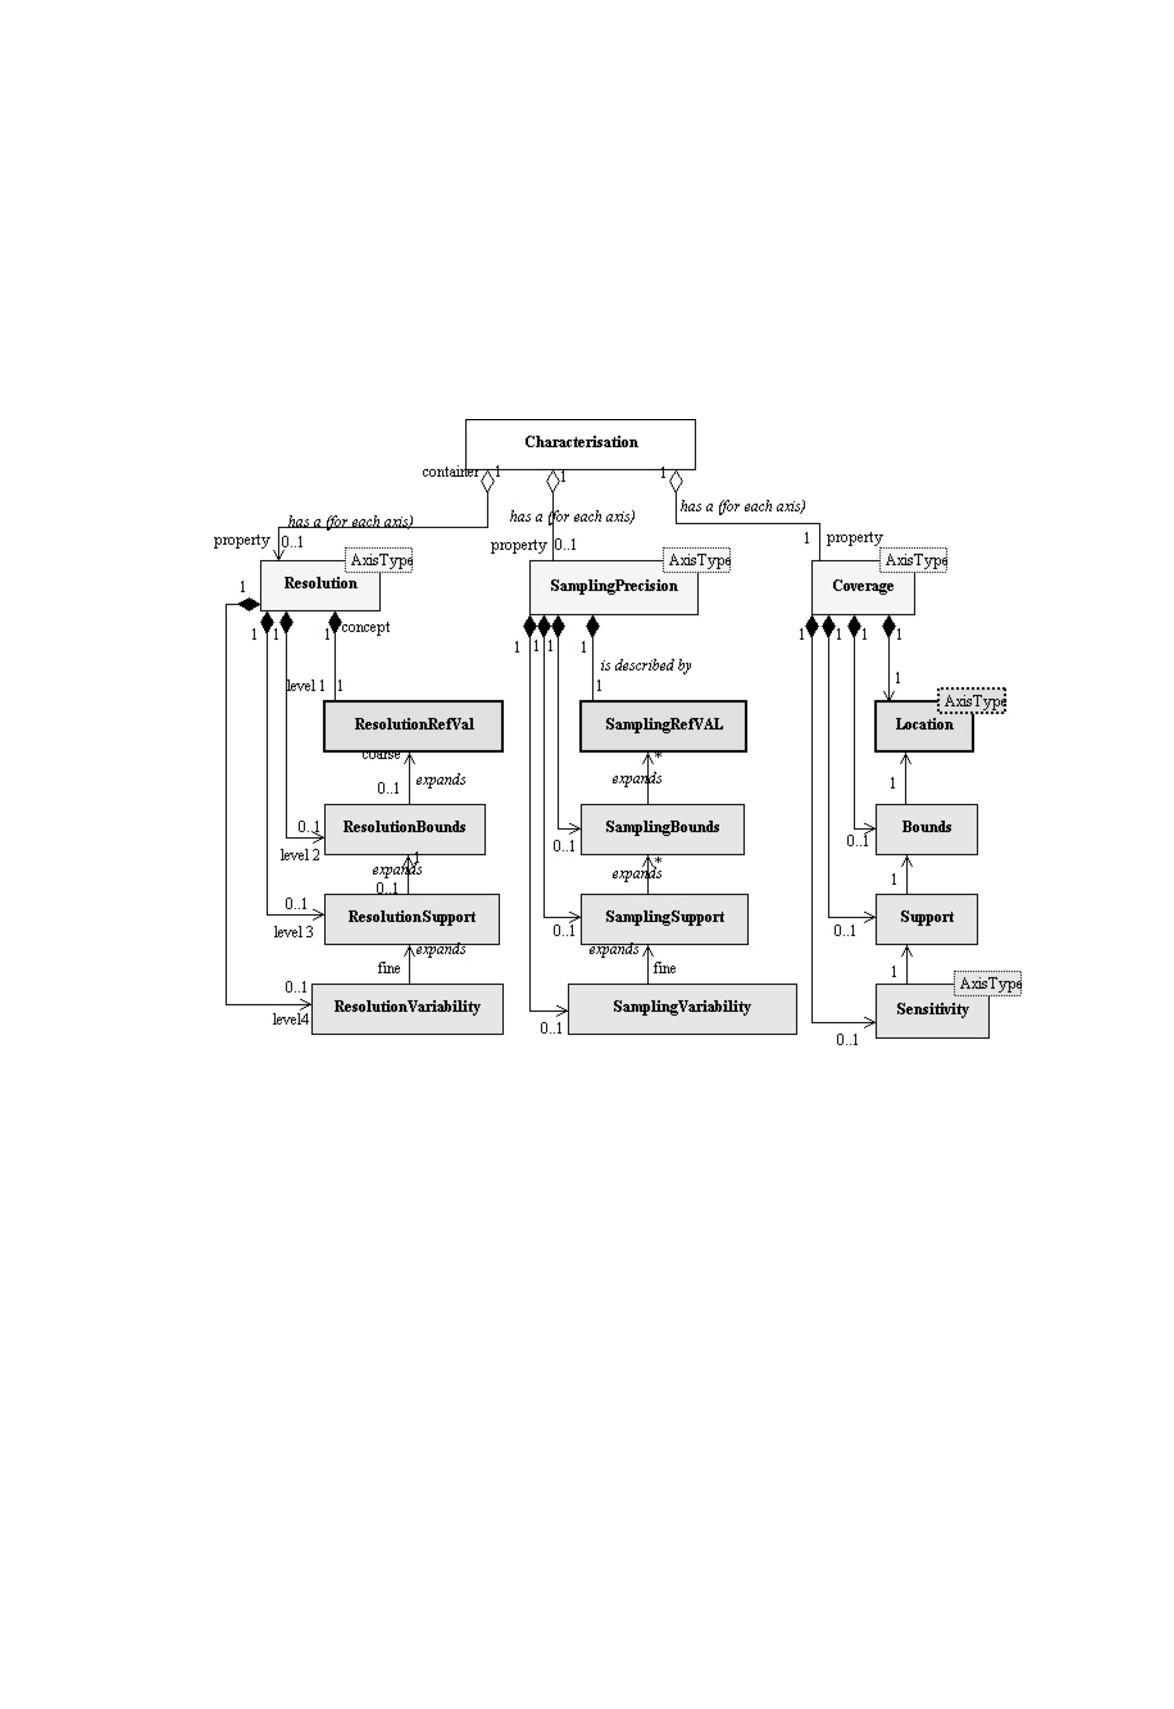
\includegraphics[width=\columnwidth]
					{fig/CharDMPerAxisProperties.pdf}
				\caption[Characterisation Data Model per axis]
				{
					Characterisation Data Model, described per axis,
					as a UML class diagram.
					Reproduced from the CharDM
					recommendation~\cite{2008dmadcrept.....L}.
				}
				\label{fig:fig_CharDMPerAxisProperties}
			\end{figure}
		
			\begin{figure}[tbp]
				\centering
					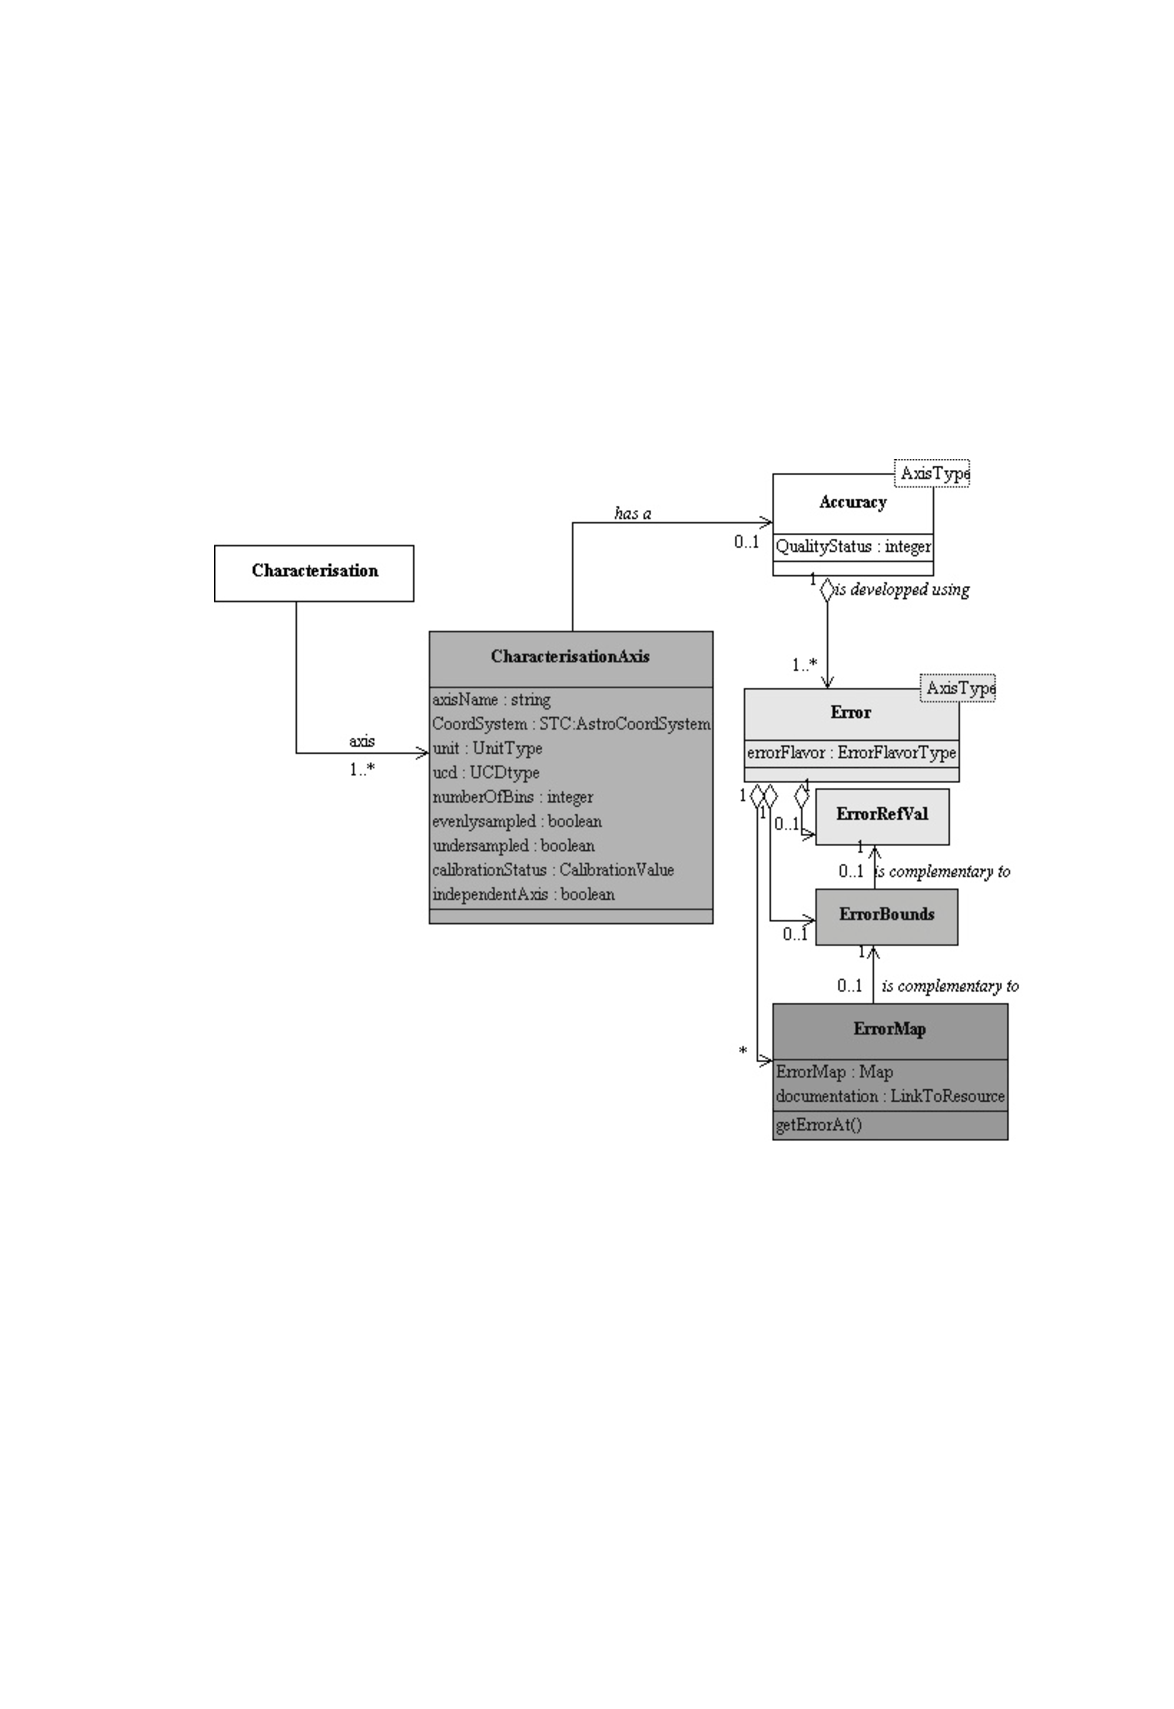
\includegraphics[width=\columnwidth]
					{fig/CharDMAccuracy.pdf}
				\caption[Accuracy class and CharacterisationAxis]
				{
					Each Characterisation instance must contain one
					or more CharacterisationAxis instances, to
					which an optional Accuracy instance can be
					attached.
					Reproduced from the CharDM
					recommendation~\cite{2008dmadcrept.....L}.
				}
				\label{fig:fig_CharDMAccuracy}
			\end{figure}
			
			 As previously said, the Characterisation data model
			(CharDM) deals with the question \emph{Where in
			parameter space is this observation?}, where the
			parameter space is comprised of the observation world
			coordinates (WCS) axis, the time axis, the spectral
			axis (and its complementary velocity axis), and the
			observable axis. Additional axes could be taken into
			account, as the structure for each axis is practically
			identical.
			
			 The CharDM (\emph{Data Model for Astronomical DataSet 
			Characterisation}~\cite{2008dmadcrept.....L}) is
			currently an IVOA Recommendation (since March 2008),
			and it covers all the sub-classes established for the
			CharDM in the ObsDM, but a few more.
			Figure~\ref{fig:fig_CharDMPerAxisProperties} shows the
			current structure of the CharDM per specified axis.
			
			 We can see that a Characterisation instance, composed
			of several CharacterisationAxis instances, each of them
			with a Coverage class, and optional SamplingPrecision
			and Resolution classes. The Coverage class must include
			a Location specification, and if they exist, both the
			SamplingPrecision and Resolution classes must provide
			reference values (RefVal). Both Location and Reference
			values can be optionally further specified by Bounds
			and Support, and a final specification in the form of
			Sensitivity for Coverage, and of Variability for
			SamplingPrecision and Resolution.
			
			 It can also be noticed that the current CharDM
			has evolved with respect to the CharDM outlined with
			the ObsDM draft: there is an additional Bounds class
			related to Coverage in each of the axes to be
			characterised.
			
			 In addition, and not shown in 
			figure~\ref{fig:fig_CharDMPerAxisProperties}, an
			Accuracy class has been added which specifies both data
			quality and errors. Figure~\ref{fig:fig_CharDMAccuracy}
			shows the Accuracy class. Each CharacterisationAxis
			instance can optionally contain an Accuracy instance,
			which is further defined by an Error class which, in
			the same spirit of the remaining Characterisation
			classes, has a RefVal, Bounds, and instead of
			Variability an ErrorMap.
			
			 We can see that the CharDM is an integral
			part of any dataset description to be made, and is as
			observation independent as possible. Indeed, the
			CharDM is also used within the VODataResource service
			description in order to characterise whole archives, or
			particular subsets of interest in the Registry.
			
		% subsection the_ivoa_characterisation_data_model (end)
		
		\subsection{Space and Time Coordinates} % (fold)
		\label{sub:space_and_time_coordinates}
			
			 The Space and Time Coordinates data
			model~\cite{2007stc..ivoa.....R} (STC) was created in
			order to have a systematic way of specifying different
			coordinate systems within the VO.
			
			 While initially the supported coordinate systems for
			VOTables and data access protocols have been Equatorial,
			with the possibility to further specify an epoch, 
			and the IAU has gone a step further with the approval
			of the International Coordinate Reference System (ICRS),
			equatorial coordinates are not
			the natural system for several astronomical disciplines,
			such as Solar System science, or Galactic studies.
			
			 The STC is both a data model (it specifies quantities
			and relationships), but also incorporates two ways of
			expressing serialisations of data model instances:
			STC-X, an XML-based STC serialisation,
			and STC-S, which is string-based and more compact
			and human readable, for use in data models
			where an XML payload cannot be delivered, or ease of
			writing is desirable.
			
			 Within the VO there are three places where the STC can
			be used: data access queries, Characterisation of
			observation Coverage in both the Spatial and Temporal
			axes, and the Object to Position resolution. However,
			for most of the existing VO services, either J2000 or
			ICRS equatorial coordinates are assumed.
			
			 The complexity of the STC stems from the very different
			coordinate systems used in astronomy, and the aim to be
			an all-encompassing effort. A glimpse of its complexity
			can be seen in figure~\ref{fig:fig_STCDM}, which shows
			the most basic STC entities\footnote{And on the STC 
			Recommendation length, which runs at 109 pages.}.
			
			Even when the STC is an IVOA Recommendation, is subject
			to analysis for better embedding in other data models
			(see the Spectrum case in the following section), and
			tools for creating/analysing STC entities are still to
			be developed.
			
			\begin{figure}[tbp]
				\centering
					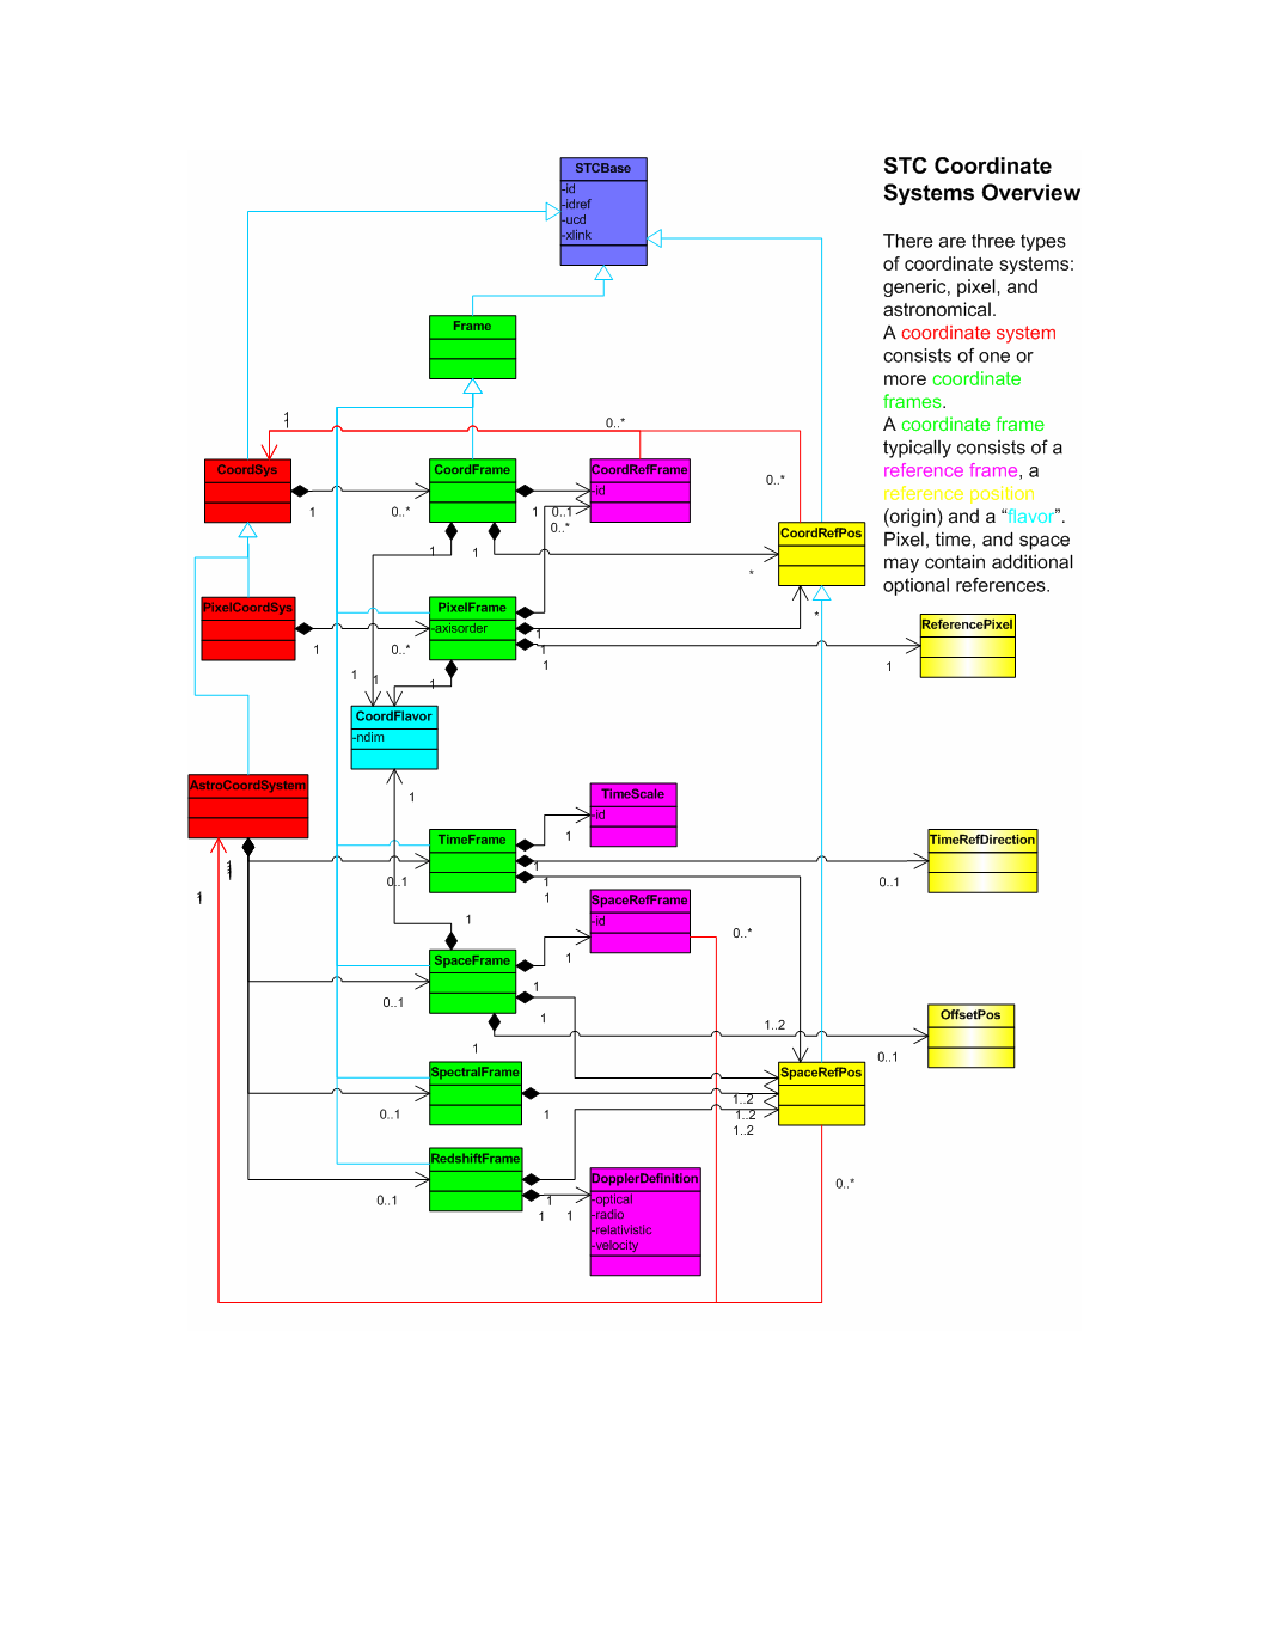
\includegraphics[width=\columnwidth]
					{fig/STCDM.pdf}
				\caption[Space and Time Coordinates data model
				overview]
				{
					An overview of the Space and Time Coordinates
					data model. Reproduced 
					from~\cite{2007stc..ivoa.....R}.
				}
				\label{fig:fig_STCDM}
			\end{figure}
			
			
		% subsection space_and_time_coordinates (end)
		
		\subsection{Spectrum} % (fold)
		\label{sub:spectrum}
			
			\begin{figure}[tbp]
				\centering
					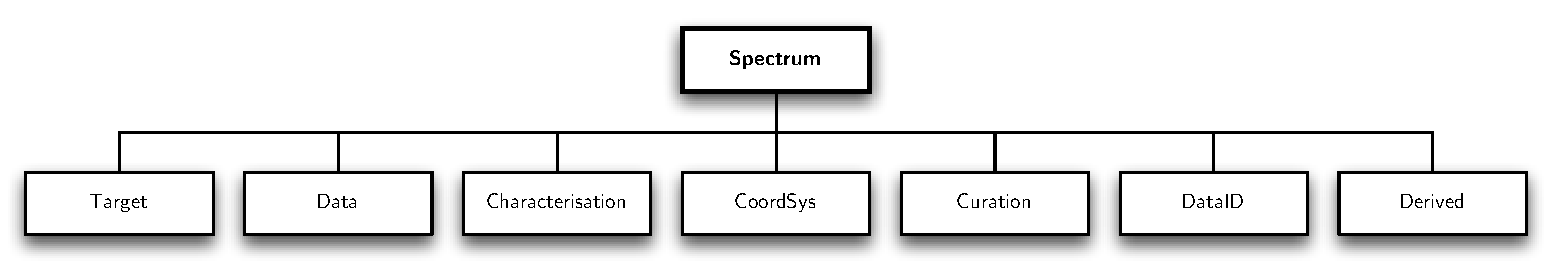
\includegraphics[width=\columnwidth]
					{fig/SpectrumDM.pdf}
				\caption[High-level overview of the Spectral DM]
				{
					High-level overview of the Spectral data model.
					The root class is the Spectrum class, which can
					compared to the Observation class in the ObsDM.
				}
				\label{fig:fig_SpectrumDM}
			\end{figure}
			
			The Spectrum data model (SpecDM) is different from the
			data models above in that it describes a particular
			data product, and not just a generic observation or an
			observation set.
			
			 Figure~\ref{fig:fig_SpectrumDM} shows the high-level
			overview of the Spectrum data model. Compared with the
			ObsDM, ---see figure~\ref{fig:fig_ObservationDM}--- and
			the CharDM ---see
			figure~\ref{fig:fig_CharDMPerAxisProperties}---, it can be
			seen that the Spectral data model is based on the
			ObsDM, without specifying a Provenance class; it
			specifies a CoordSys class separate from Target, and
			also a DataID (a simplified data curation for a
			particular entity); and a Derived class for holding
			information which does not belong to the Spectrum, but
			can be derived from it under several assumptions, such
			as the Signal-to-Noise Ration (SNR), Redshift and
			Amplitude variability.
			
			 Due to the already mentioned complexity of the STC,
			the SpecDM uses a simplified version of STC-S entities
			to describe spatial regions (circles and poligons for
			the SpecDM) and temporal coordinates.
			
			 There are many different techniques to obtain spectra,
			and each of them produces a different data product.
			The most important difference concerns on whether the
			spectrum is obtained by a diffraction or refraction
			method, which provides a sampling on wavelength; or if
			the spectrum is obtained via a Fourier transform
			method (from the Fourier transform of an autocorrelation
			signal, for instance), which provides a sampling on
			frequency. As frequency and wavelength for
			electromagnetic radiation are linked by a non-lineal 
			equation ($\lambda = c\nu^{-1}$), it is very important
			for astronomical data processing applications to
			treat each case differently\footnote{To the point that
			the SpecDM recommends using different Spectrum entities
			for spectra which are available both with a frequency
			and a wavelength scale.}.
			
			 The SpecDM has reached IVOA Recommendation status, but
			its Characterisation class is still not fully
			compatible with the last version of the CharDM, as
			sanctioned as IVOA Recommendation. Debate is still
			open on how to use it for time series, instead of the
			time series provisions included in the STC data model.
			Finally, the Spectrum class can only identify one
			single spectrum. Work has yet to start on the
			Spectral Associations data model, in order to describe,
			for instance, On-The-Fly spectra, 3D IFU spectra, or
			any other multidimensional datasets where one of the
			dimensions is frequency, wavelength or velocity.
			
		% subsection spectrum (end)
		
		%\subsection{The DAL model} % (fold)
		%\label{sub:the_dal_model}
		%	
		%	We have mentioned
		%	---section~\ref{sec:role_of_data_models_in_the_vo}---
		%	the DAL data model.
		%	
		%	This simplified model, which 
		%	
		%% subsection the_dal_model (end)
		
	% section existing_ivoa_data_models (end)
	
	\section{Other astronomical data modelling efforts} % (fold)
	\label{sec:other_astronomical_data_modelling_efforts}
		
		Apart from the IVOA data models mentioned above, we have
		reviewed some other data models relevant to astronomical
		observations' data modelling, or data modelling for
		radio astronomical archives.
		
		The only IVOA Note on radio astronomy data prior to the
		publication of the RADAMS was the \emph{Data model for
		Raw Radio Telescope} by Lamb and
		Power~\cite{LamPow0310IVOA}.
		
		Many aspects of our work ---specially controlled
		vocabularies, and the extensibility to interferometry---
		were initially based upon this model.
		
		\newcommand{\asdmurl}[0]
		{http://aramis.obspm.fr/~alma/ASDM/ASDMEntities/}
		Other models reviewed include the data model used for
		publication of the Australian Telescope Compact Array
		(ATCA)~\cite{2006astro.ph..1354}
		archive\urlnote{http://atoa.atnf.csiro.au/}, the scientific
		archive domain model of the National Optical Astronomy
		Observatory (NOAO)~\cite{War04NOAO}
		archives\urlnote{http://archive.noao.edu/nsa/}, and the
		ALMA Science Data
		Model\urlnote{\asdmurl}~\cite{2006ASPC..351..627V}.
		
		A special mention is made of the MPEG-7 and MPEG-21
		overview documents~\cite{Bormans:fk, Martinez:uq},
		available in web-page form at
		\url{http://www.chiariglione.org/}, used as the basis for
		our Policy and Curation sub-models.
		
		
	% section other_astronomical_data_modelling_efforts (end)
	
	\section{Conclusions} % (fold)
	\label{sec:dm_conclusions}
		
		Within the VO, data to be delivered must be described in
		the most complete possible way so that automated selection
		and manipulation tools can rely on that description in
		order to manipulate, select, and ultimately provide
		\emph{understanding} of the described data.
		
		 Both the data themselves and the metadata need to conform
		to a common data model, in order to make interoperability
		between different systems possible. Those data models are
		governed by the IVOA DM WG.
		
		 The only observation-related data model already in
		Recommendation stage is the SpecDM. The other data models
		having reached Recommendation status are the STC data model,
		and the CharDM.
		
		 The SpecDM shows that it is possible to use the ObsDM as
		a template to create an observation-specific data model,
		and both the CharDM and the STC have shown their modularity
		in order to be embedded in other data models. However, 
		STC entities are usually simplified before being properly
		used.
		
		 In order to create a complete VO-compliant data model
		which can hold all kinds of radio observations from
		different single-dish observatories we will provide, then:
		
		\begin{description}
			\item[Compatibility with existing and/or proposed data
			models] Any VO-com\-pli\-ant da\-ta mo\-del should make
			use of existing and recommended IVOA data models, and
			should try to fit themselves within the data model most
			related to the kind of data to be described.
			
			\item[Use of existing data models in comparable
			e-Science disciplines] The Virtual Observatory is
			one example of an e-Science based discipline: the
			main success of the VO comes from the federation of
			disperse datasets, and their aggregation through
			network access protocols. As such,
			it would be wise to make use of the existing e-Science
			middleware and conventions for non astronomy-specific
			parts of the system.
			
			\item[Support for spectral associations] 
			The SpecDM provides support for spectral measurements,
			but there is no way to relate spectra taken from
			On-The-Fly observations, or spectra extracted from a
			radio data cube, or maps of continuum measurements.
			This support is added to the RADAMS by combining
			the CharDM and Packaging.
			
			\item[Specification of missing classes] 
			The ObsDM proposed classes for dealing with data
			access Policies, data Provenance, and data Packaging, 
			while the CharDM proposed a Sensitivity class. A
			data model for radio astronomical observations would
			need to provide definitions for such classes.
			
			\item[Support for radio astronomical observing modes]
			There are widely different observing modes in radio
			astronomical, single dish, observatories. A VO data
			model for them would have to support them.
			
			\item[Extensibility for radio interferometric
			observations] Most of the data model details can be
			generalised for radio interferometric observations,
			and where possible the way to extend the data model
			in order to support interferometric observations is
			made explicit.
		\end{description}
		
		We will address these requirements in the following chapters.
		
	% section dm_conclusions (end)
	
	%% section radio_dm_needs (fold)
	%\section{Needs for a radio astronomical observation data model} 
	%\label{sec:radio_dm_needs}
	%
	%	Radio astronomical observations can be defined as those
	%	performed in the radio band,
	%	%(from 13~MHz to the 1~THz range),
	%	and for single dish radio telescopes can be classified as:
    %
	%	\begin{description}
	%		\item[Total flux] measures all the incoming energy in
	%		the receiver's bandwidth, typically measured by
	%		non-coherent receivers, or derived by integration of
	%		the signal received by coherent receivers. This kind of
	%		measurement is also called continuum measurement.
	%		
	%		\item[Spectrum] a frequency-dependent energy
	%		distribution across a given bandwidth, and with a given
	%		resolution.
	%	\end{description}
	%	
	%	As there are emission sources other than the astronomical
	%	source being studied, a reference signal must be obtained
	%	and subtracted form the total signal coming from the source
	%	of interest. The reference signal can be obtained:
	%	
	%	\begin{description}
	%		\item[By switching positions] The radio sky is
	%		typically obscure. By moving away from a radio source,
	%		we are effectively measuring the sky contribution.
	%		There are several ways of switching positions: changing
	%		to an absolute, fixed sky position, or switching to a
	%		position which is at a certain angular distance from
	%		the observed position, and keeps the distance while
	%		mapping across a source. Further divisions can be made
	%		on how is the switching performed: by moving the
	%		antenna, by moving the secondary mirror (always a
	%		relative position switching), or by using a chopper
	%		wheel, for instance.
	%		
	%		\item[By switching frequency] Radio sources typically
	%		follow a power law in their intensity, while sky noise
	%		follows a flat distribution. By switching to lower
	%		frequencies, we can sample the amount of sky noise,
	%		which can then be subtracted of our intended signal.
	%		
	%	\end{description}
	%	
	%	Another difference is on antenna tracking:
	%	
	%	\begin{description}
	%		\item[Fixed tracking] with fixed tracking, the antenna
	%		movement is just enough to track a single position
	%		in celestial coordinates; only data from a single
	%		coordinate (other than reference
	%		measurements) are obtained.
	%		
	%		\item[Point to point tracking] the antenna can be pointed
	%		to different coordinates, and obtain data from each of
	%		them.
	%		
	%		\item[On-the-fly tracking] in this case, the antenna
	%		follows a pattern across the sky, and measurements are
	%		continually recorded, so that there is not a single
	%		position which can be attributed to each measurement,
	%		but instead the measurement is assigned to a segment
	%		of the sky. However, the advantage of this kind of
	%		tracking is the faster mapping of the sky with a
	%		similar signal to noise ration. In any case, the
	%		paths described across the sky need to be specified.
	%		
	%		\item[Solar system tracking] the tracking methods
	%		imply positions are fixed in the celestial sphere, but
	%		for solar system objects the object orbit has to be
	%		computed, and the tracking system made to follow that
	%		orbit, instead of just tracking the movement of the sky.
	%		
	%	\end{description}
	%	
	%	In brief, a data model for radio astronomical observations
	%	needs to provide metadata for:
	%	
	%	\begin{itemize}
	%		\item Project related information, in order to be able
	%		to query on PI, or a whole observation project.
	%		
	%		\item Observation characterisation information: where
	%		in the celestial sphere, time, bandwidth and observed
	%		flux axes is comprised an observation.
	%		
	%		\item Telescope and instrument setup information.
	%		
	%		\item Ambient conditions information.
	%		
	%		\item Processing steps performed on the selected data.
	%		This includes identifying the final data product
	%		being delivered, and the way the reference signal is
	%		obtained.
	%	\end{itemize}
	%	
	%	But, in addition, the following needs have also to be
	%	fulfilled:
	%	
	%	\begin{itemize}
	%		\item Provide data access policy information. We will
	%		include it in a Policy class, and we will take
	%		inspiration from the Policy classes available for
	%		accessing restricted media, such as those proposed by
	%		the MPEG-7 and MPEG-21 standards.
	%		
	%		\item 
	%	\end{itemize}
	%
	%% section radio_dm_needs (end)


% chapter data_modelling_in_the_vo (end)

